\begin{bquote}{Thief of Time, Terry Pratchett\nocite{pratchett2001}}
  % hack to stop the displayquote from eating the [
  {[}\dejafu{} is] A martial art in which the user's limbs move in time
  as well as space, [\ldots] It is best described as ``the feeling
  that you have been kicked in the head this way before''.
\end{bquote}

\noindent
Tools are necessary to test concurrency, the standard approach does
not suffice.  In this chapter we present and evaluate \dejafu{}, our
library for testing concurrency in Haskell.  We discuss the scope of
the tool~\sref{dejafu-scope} and present our abstraction over the GHC
Haskell concurrency functionality~\sref{dejafu-monadconc}.  We then
show an example of a small logic puzzle which we can represent as a
concurrent program~\sref{dejafu-100}.  We explain how programs using
our abstraction are executed~\sref{dejafu-execution} and
tested~\sref{dejafu-testing}, and argue the correctness of the testing
approach~\sref{dejafu-correctness}.  We present three case
studies~\sref{dejafu-casestudies}, evaluate the usefulness of
\dejafu{} for testing pre-existing code~\sref{dejafu-evaluation}, and
finally draw conclusions and present further
work~\sref{dejafu-conclusions}.

This chapter is derived from our previous work \cite{walker2015} and
\cite{YCS-2016-503}.

\section{Scope}
\label{sec:dejafu-scope}

We aim to support most of the functionality of GHC’s concurrency API, as made
available through the Control.Concurrent and Control.Exception module
hierarchies, which does not unavoidably require support from the runtime system.

In particular, we do not support:

\begin{itemize}
\item Blocking a thread until a file descriptor becomes available, as this
  introduces an additional source of nondeterminism.
\item Throwing an exception to a thread if it becomes deadlocked, as we cannot
  reliably detect deadlock involving only a subset of threads without support
  from the garbage collector.
\item Querying which capability (OS thread) a Haskell thread is running on, as
  this introduces an additional source of nondeterminism.
\end{itemize}

We also do not yet support \emph{bound threads}: a Haskell thread which will
always run on the same, unique, OS thread.  Bound threads are essential for
using the FFI to call libraries which use thread-local state, to ensure the
Haskell thread always sees its state and never the state of another thread.  We
have a prototype implementation, which is not yet present in a released version
of \dejafu{}\footnote{\url{https://github.com/barrucadu/dejafu/issues/126}}.

\section{Abstracting over \texttt{IO}}
\label{sec:dejafu-monadconc}

Recall from \cref{sec:sct-fundamentals} that there are three ways of
implementing a concurrency testing tool:

\begin{itemize}
\item Override the concurrency primitives of the programming language.
\item Instrument the source program.
\item Instrument the compiled program.
\end{itemize}

We adopt the first approach in \dejafu{}.  Haskell's typeclass machinery lets us
specify an interface for concurrency, and to provide different concrete
implementations.  There is one implementation using the \verb|IO| type and the
standard functions; there is another using our own type, based on continuations
which we can inspect.

\begin{listing}
  \begin{minted}{haskell}
class (Monad m, {- other constraints omitted -}) => MonadConc m where
  type MVar m :: * -> *
  -- other types omitted

  newEmptyMVar :: m (MVar m a)
  newEmptyMVar = newEmptyMVarN ""

  newEmptyMVarN :: String -> m (MVar m a)
  newEmptyMVarN _ = newEmptyMVar

  putMVar  :: MVar m a -> a -> m ()
  readMVar :: MVar m a -> m a
  takeMVar :: MVar m a -> m a
  -- other operations omitted
  \end{minted}
  \caption{A fragment of the \texttt{MonadConc} typeclass.}\label{lst:monadconc}
\end{listing}

We call our typeclass \verb|MonadConc| for monads which can do concurrency,
\cref{lst:monadconc} shows a fragment.  When defining an instance of this class,
the programmer must supply concrete types for the abstract types in the
interface.  They must also supply implementations of, at least, all undefined
operations.  Some operations have default definitions: for example, there are
two ways of constructing an empty \verb|MVar|.  One way takes a name, which is
displayed in debugging information, the other does not.  Each is defined in
terms of the other, and so the programmer must supply at least one.

\begin{listing}
  \begin{minted}{haskell}
instance Monad n => MonadConc (ConcT r n) where
  type MVar (ConcT r n) = MVar r
  -- other types omitted

  newEmptyMVarN n = toConc (ANewMVar n)

  putMVar  var a = toConc (\c -> APutMVar var a (c ()))
  readMVar var   = toConc (AReadMVar var)
  takeMVar var   = toConc (ATakeMVar var)
  -- other operations omitted
  \end{minted}
  \caption{A fragment of the \texttt{MonadConc} testing implementation.}\label{lst:mvarops}
\end{listing}

The type for our testing implementation is called \verb|ConcT r n|, which is a
monad that has access to \emph{references} of type \verb|r| in a monad of type
\verb|n|.  \Cref{lst:mvarops} shows the implementation of \cref{lst:monadconc} for
this type.  Each concurrency operation is of the same form: we take the
arguments and wrap them up inside a data structure whose final argument is a
continuation, which is then converted into a \verb|ConcT| value.

A concurrent computation is just a large value, where we can inspect each
``step'' of the computation by looking at the data constructor used.
Constructors mostly correspond to operations in the \verb|MonadConc| class
(there are also a few extra).  We call these constructors \emph{primitive
  actions}.  A full listing is available in \cref{app:primops-conc}.

We make a few departures from the semantics of the \verb|IO| monad where
necessary:

\begin{itemize}
\item The \verb|getNumCapabilities| operation allows the programmer to query the
  number of capabilities.  During testing, we return ``2'', despite executing
  everything in the same OS thread.  This is to avoid special-case behaviour for
  one capability, which may reduce concurrency.
\item Runtime errors, such as pattern match failures, can be caught as
  exceptions inside \verb|IO|.  As there is no non-\verb|IO| way to do the same,
  \dejafu{} cannot.
\item The \verb|threadDelay| operation is required to yield the thread, but not
  necessarily to delay it.  This is because it is not clear how to incorporate
  time into the systematic concurrency testing model.
\end{itemize}

There is more to \verb|IO| than concurrency and exceptions.  \dejafu{} supports
testing computations with embedded \verb|IO| actions provided that the
programmer ensures that the \verb|IO| action is atomic; that it is deterministic
when executed with a fixed schedule; and that it does not block on the action of
another thread.  Failing to meet any of these conditions may lead to incomplete
testing.

\section{The 100 Prisoners Problem}
\label{sec:dejafu-100}

There's a popular logic puzzle which goes something like this:

\begin{displayquote}
  There are 100 prisoners in solitary cells.  There's a central living
  room with one light bulb.  No prisoner can see the light bulb from
  their own cell.  Everyday, the warden picks a prisoner equally at
  random, and that prisoner visits the living room.  While there, the
  prisoner may toggle the bulb.  The prisoner also has the option of
  asserting that all 100 prisoners have been to the living room.  If
  this assertion is false, all 100 prisoners are shot.  However, if
  true, all prisoners are set free.  Thus, the assertion should only
  be made if the prisoner is 100\% certain of its validity.  The
  prisoners are allowed to get together one night in the courtyard, to
  discuss a plan.  What plan should they agree on, so that eventually,
  someone will make a correct assertion?
\end{displayquote}

We can express this puzzle as a concurrency problem: the warden is the
scheduler, each prisoner is a thread, and when the program terminates
every prisoner should have visited the living room.  So if every
thread (prisoner) that is forked is scheduled (taken to the room),
then the prisoners are successful.  \dejafu{} can give us an execution
trace.  So, given some way of setting up the prison, we can ask
\dejafu{} to execute it and then examine the returned traces to
discover if the prisoners are successful.

\subsection{The ``Good Enough'' Solution}

One school of thought says to just wait for three years, because by
then it's unlikely that any single prisoner had never visited the
room.  In fact, w would expect each prisoner to have been to the room
ten times by then.  \Cref{lst:100good} shows an implementation of this
strategy, and \cref{tbl:100rand} shows how the prisoners fare over 100
random executions.

\begin{table}
  \centering
  \begin{tabular}{l|rrrrrrrr} \toprule
    Prisoners          &   1 &   2    &   3    &   4    &   5    &   6    &   7    &   8 \\
    Successes          & 100 & 100    & 100    & 100    & 100    & 100    & 100    & 100 \\
    Failures           &   0 &   0    &   0    &   0    &   0    &   0    &   0    &   0 \\
    Avg.\@ Room Visits &   2 &  18.35 &  31.92 &  43.52 &  55.88 &  67.37 &  77.05 &  90.40 \\ \bottomrule
  \end{tabular}
  \caption{The behaviour of the good enough solution.}\label{tbl:100rand}
\end{table}

After waiting $10 n$ days, where $n$ is the number of prisoners, the
chance that any one prisoner has been consistently missed is
$\left(1 - \frac{1}{n}\right)^{10n}$.  This is roughly 0.004\% for 100
prisoners, and converges to $\frac{1}{e^{10}}$.

\subsection{The Perfect Solution}

Perhaps our prisoners are more cautious, and a 0.004\% chance of death
is too much.  They want to be certain of their success.  A slow but
simple strategy is for the prisoners to nominate a leader.  Only the
leader can declare to the warden that everyone has visited the room.
Whenever a prisoner other than the leader visits the room, if the
light is on, they do nothing; otherwise, if this is their first time
in the room with the light off, they turn it on, otherwise they leave
it.  Whenever the leader enters the room, they turn the light off.
When the leader has turned the light off 99 times, they tell the
warden that everyone has visited.  \Cref{lst:100perfect} shows an
implementation of these behaviours.

\begin{listing}
\begin{sublisting}{\textwidth}
\begin{minted}{haskell}
leader :: MonadConc m => Int -> TVar (STM m) Int -> m ()
leader numPrisoners days = atomically $ do
  numDays <- readTVar days
  when (numDays < (numPrisoners - 1) * 10) retry

notLeader :: MonadConc m => TVar (STM m) Int -> m ()
notLeader days = forever $ atomically (modifyTVar days (+1))

prison :: MonadConc m => Int -> m ()
prison numPrisoners = do
  days <- atomically (newTVar 0)
  for_ [1..numPrisoners-1] (\_ -> fork (notLeader days))
  leader numPrisoners days
\end{minted}
\caption{The good enough solution: just wait a long time and gamble.}\label{lst:100good}
\end{sublisting}

% [layout hack]: no gap between the listings otherwise
\vspace{2.5em}

\begin{sublisting}{\textwidth}
\begin{minted}{haskell}
data Light = IsOn | IsOff

leader :: MonadConc m => Int -> TVar (STM m) Light -> m ()
leader numPrisoners light = go 0 where
  go counter = do
    counter' <- atomically $ do
      state <- readTVar light
      case state of
        IsOn -> do
          writeTVar light IsOff
          pure (counter + 1)
        IsOff -> retry
    when (counter' < prisoners - 1)
      (go counter')

notLeader :: MonadConc m => TVar (STM m) Light -> m ()
notLeader light = do
  atomically $ do
    state <- readTVar light
    case state of
      IsOn  -> retry
      IsOff -> writeTVar light IsOn
  forever yield

prison :: MonadConc m => Int -> m ()
prison numPrisoners = do
  light <- atomically (newTVar IsOff)
  for_ [1..numPrisoners-1] (\_ -> fork (notLeader light))
  leader numPrisoners light
\end{minted}
\caption{The perfect solution: nominate a leader, who waits until they are certain that everyone has been in the room.}\label{lst:100perfect}
\end{sublisting}
\caption{Two solutions for the 100 prisoners problem.}\label{lst:100sols}
\end{listing}

We can satisfy ourselves that this works for all cases by using
\dejafu{}'s systematic concurrency testing functionality, which is a
combination of dynamic partial-order reduction and schedule bounding.
\Cref{tbl:100slow} shows how the number of attempts and average room
visits grows as the number of prisoners increases.

\begin{table}
  \centering
  \begin{tabular}{l|rrr} \toprule
    Prisoners          & 1 & 2 &    3 \\
    Schedules          & 1 & 5 & 2035 \\
    Avg.\@ Room Visits & 2 & 7 &  133 \\ \bottomrule
  \end{tabular}
  \caption{Schedule growth with increasing prisoner numbers.}\label{tbl:100slow}
\end{table}

This doesn't scale well.  Our algorithm is a really bad case for
concurrency testing: every thread is messing with the same shared
state, so \dejafu{} has to try all the orderings.  Taking another look
at our prisoners, we can see two things which a human would use to
decide whether some schedules are redundant or not:

\begin{enumerate}
\item If we adopt any schedule other than alternating leader /
  non-leader, threads will block without doing anything.  So we should
  alternate.
\item When a non-leader has completed their task, they will always
  yield.  So we should never schedule a prisoner who will yield.
\end{enumerate}

\dejafu{} can't make use of (1).  It could be inferred \emph{if}
\dejafu{} were able to compare values inside \verb|TVar|s.  We cannot
do that without putting an \verb|Eq| constraint on \verb|writeTVar|,
however.

\dejafu{} \emph{can} make use of (2).  \dejafu{} already bounds the
maximum number of times a thread can yield, so that it can test
constructs like spinlocks.  This is called \emph{fair bounding}.  The
default bound is 5, but if we set it to 0 \dejafu{} will never
schedule a thread which is going to yield.  \Cref{tbl:100fast} shows how
the number of schedules and average room visits grows with this
change.

\begin{table}
  \centering
  \begin{tabular}{l|rrrrrr} \toprule
    Prisoners          & 1 & 2 & 3   &  4   &    5 &      6 \\
    Schedules          & 1 & 1 & 4   & 48   & 1536 & 122880 \\
    Avg.\@ Room Visits & 2 & 4 & 7.5 & 11.5 &   16 &     21 \\ \bottomrule
  \end{tabular}
  \caption{Schedule growth with increasing prisoner numbers (improved).}\label{tbl:100fast}
\end{table}

This is better, but still scales poorly.  The prisoners are stepping
on each other's toes and causing needless work.  This is probably as
good as we can do without adding some extra primitives to \dejafu{} to
optimise the case where we have an \verb|Eq| instance available.

It's not the end for systematic testing, however.  Empirical
studies\cite{thomson2014} have found that many concurrency bugs can be
exhibited with only two or three threads.  Furthermore, most
real-world concurrent programs don't have every single thread
operating on the same bit of shared state.

\section{Executing Concurrent Programs}
\label{sec:dejafu-execution}

Concurrent computations are expressed in terms of a continuation monad.  As we
have noted previously, operations in the \verb|MonadConc| typeclass are
represented by a type of ``primitive actions'', where each action describes some
effect and has a continuation.  This is the \verb|Action| type.  Each thread of
execution is terminated by a distinguished \emph{stop} primitive, which has no
continuation and signals successful completion.

\begin{listing}
  \begin{minted}{haskell}
newtype M n r a = M { runM :: (a -> Action n r) -> Action n r }

instance Functor (M n r) where
  fmap f m = M (\c -> runM m (c . f))

instance Applicative (M n r) where
  pure x  = M (\c -> AReturn (c x))
  f <*> v = M (\c -> runM f (\g -> runM v (c . g)))

instance Monad (M n r) where
  return  = pure
  m >>= k = M (\c -> runM m (\x -> runM (k x) c))

#if MIN_VERSION_base(4,9,0)
  fail = Fail.fail

instance Fail.MonadFail (M n r) where
#endif
  fail e = M (\_ -> AThrow (MonadFailException e))
  \end{minted}
  \caption{The \dejafu{} continuation monad.}\label{lst:m}
\end{listing}

\Cref{lst:m} gives the definition and typeclass instances of the \dejafu{}
continuation monad.  The \verb|Functor| instance allows applying a function to
the input of the continuation.  The \verb|Applicative| instance allows injecting
a pure value into the \verb|M| type, by constructing a continuation which
consumes this value.  It also allows extracting a function from one computation,
a value from another, and applying them.  The \verb|Monad| instance allows
sequencing.  Finally, the \verb|MonadFail| instance alows signalling a pattern
match failure in a monadic expression.  \dejafu{} aims to support the latest
three major releases of GHC, and so we use conditional compilation here.

\paragraph{Operational Semantics}
We give an operational semantics for Haskell concurrency in the form of a step
function on primitive actions.  Given the current state, which we call the
\emph{context}, the identifier of the chosen thread, and its primitive action,
we either indicate a failure condition, or produce a new state; in both cases we
return a log of what happened, to put into the execution trace returned to the
user.

Our context value does not contain a heap, instead we use Haskell mutable
references directly.  This means that executing our step function has
side-effects, and in general contexts should not be re-used.  This is not a
limitation in practice because we never want to re-use contexts.  We could
include the heap state in our context, by using a heterogeneous map
type\footnote{Like the \inlpackage{vault} library.}, however the additional
indirection both increases allocation, and reduces the efficacy of garbage
collection.  By using Haskell mutable references directly, when all copies of a
reference fall out of scope, the referenced value can be garbage collected;
whereas if we model references as keys into a heap, then such data can never be
freed, as we cannot tell when it is safe to delete something from our heap.

\begin{listing}
\begin{minted}{haskell}
pure id <*> v
  = M (\c -> AReturn (c id)) <*> v
  = M (\c -> runM (M (\c -> AReturn (c id))) (\g -> runM v (c . g)))
  = M (\c -> (\c -> AReturn (c id)) (\g -> runM v (c . g)))
  = M (\c -> AReturn ((\g -> runM v (c . g)) id))
  = M (\c -> AReturn (runM v (c . id)))
  = M (\c -> AReturn (runM v c))
 /= v
\end{minted}
  \caption{Expansion of the \texttt{Applicative} identity law.}\label{lst:areturn}
\end{listing}

\paragraph{Nonterminating Executions}
\dejafu{} is only able to make scheduling decisions at the level of primitive
actions, which means that if evaluating a primitive action does not terminate,
\dejafu{} will hang.  We deliberately break the \verb|Applicative| identity law,
that \verb|pure id <*> v = v| for all \verb|v| (\cref{lst:areturn}), to make some
programs more defined than they otherwise would be.  Consider this small
program:

\begin{minted}{haskell}
test = forever (pure "loop") where
  forever mx = mx >> forever mx
\end{minted}

Neither \verb|(>>)| nor \verb|forever| correspond to primitive actions, so they
cannot be pre-empted.  If \verb|pure| did not correspond to a primitive action
either, then that expression would cause \dejafu{} to loop forever, trying to
find the continuation.  This is an unhelpful result.  By breaking the laws and
introducing a way to interrupt the \verb|forever| computation, \dejafu{} can
instead report that trying to test this program exceeds the execution length
limit\footnote{\url{https://github.com/barrucadu/dejafu/issues/27}\\\url{https://github.com/barrucadu/dejafu/issues/113}}.

\paragraph{Scheduling}
The choice of which thread to execute is made by a scheduler function, which is
supplied by the user.  The scheduler is called even if there is only one
runnable thread, to keep things simple.  A scheduler, shown in
\cref{lst:scheduler}, is a stateful function which is given the previous action
and the runnable threads, which possibly returns a thread to run.  If no thread
is returned, the computation is aborted.  This is used to implement schedule
bounding.  The state is used to implement partial-order reduction and random
scheduling: in the former, the state is a list of scheduling decisions designed
to put the system into an unseen state; in the latter, the state is a random
number generator.

\begin{listing}
  \begin{minted}{haskell}
newtype Scheduler state = Scheduler
  { scheduleThread
    :: Maybe (ThreadId, ThreadAction)
    -> NonEmpty (ThreadId, Lookahead)
    -> state
    -> (Maybe ThreadId, state)
  }
  \end{minted}
  \caption{The \dejafu{} \texttt{Scheduler} type.}\label{lst:scheduler}
\end{listing}

\paragraph{Success and Failure}
When testing concurrent computations, we are interested in both
success and failure.  If a computation succeeds and returns a value,
we want to know that; if it fails and deadlocks, we also want to know
that.  The result of a single execution of the program is an
\verb|Either Failure result| value, where the \verb|Failure| type is
an enumeration of error conditions that \dejafu{} can detect, and the
\verb|result| type is the result in the successful case.

\subsection{Software Transactional Memory}

Transactions allow the atomic execution of a sequence of operations involving
\verb|TVar|s, transactional variables.  Unlike operations on \verb|CRef|s or
\verb|MVar|s, transactions are composable and the whole remains atomic.

We express transactions in a similar way to concurrent programs: as a
continuation monad over a primitive action type.  A complete listing of actions
is available in \cref{app:primops-stm}.  As \dejafu{} drives the execution of a
concurrent program, it is possible to have arbitrarily complex effects which
appear atomic to the program under test.  In particular, we ensure atomicity by
executing concurrency primitive actions sequentially, ensuring that no two
transactions (or no two actions of any form) can interfere.

The STM primitive actions have a small-step operational semantics defined as a
step function.  Like the small-step semantics of the concurrency primitive
actions, this does not include a model of the heap.  However, as transactions
are atomic, we only care about the big-step behaviour.  This simplifies some
aspects of the implementation, but means that we cannot cope with nonterminating
transactions at all, whereas we can abort concurrent programs which have taken
too many steps.

A transaction evaluates to some success value, a thrown exception, or an abort.
If successful, it may also mutate some transactional variables as a side-effect;
otherwise it does not.  If it evaluates to a thrown exception, we throw the
exception in the thread performing the transaction.  If it evaluates to an
abort, we block the thread performing the transaction until at least one
\verb|TVar| read in the transaction is mutated by another thread.

\subsection{Relaxed Memory}

There are three memory models supported in \dejafu{}:

\begin{description}
\item[Sequential Consistency] This model is the most intuitive.  A program
  behaves as a simple interleaving of the actions in different threads.  When a
  \texttt{CRef} is written to, that write is immediately visible to all
  threads.

\item[Total Store Order (TSO)] Each thread has a write buffer.  A thread sees
  its writes immediately, but other threads will only see writes when they are
  \emph{committed}, which may happen later.  Writes by the same thread are
  committed in program order.

\item[Partial Store Order (PSO)] A relaxation of TSO where each thread has a
  write buffer for each \verb|CRef|.  Writes to different \verb|CRef|s by the
  same thread are not necessarily committed in program order.
\end{description}

The default memory model for testing is TSO, as that most accurately models the
behaviour of modern x86 processors\cite{owens2009}.  The use of a relaxed memory
model can require a much larger number of schedules when its effects are at
play.

\paragraph{Write Buffering}
We model relaxed memory by introducing buffers for thread writes.  When a thread
writes to a \verb|CRef|, the write is appended to its buffer.  When a thread
reads from a \verb|CRef|, it reads the value of the newest write in its buffer,
or the most recently committed value if the buffer is empty.  After a write is
committed, it is removed from its buffer.  Any non-empty buffer may have a write
committed, but only the oldest write in a buffer may be committed.  \Cref{fig:wb}
shows the arrangement of buffers for the three memory models in a system with
two threads and two \verb|CRef|s.

\begin{figure}
  \centering
  \begin{subfigure}{0.3\textwidth}
    \centering
    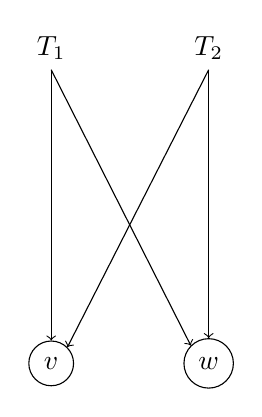
\begin{tikzpicture}
      \node (t1) at (-1,0) {$T_1$};
      \node (t2) at (1,0)  {$T_2$};
      \node (v) [draw,shape=circle] at (-1,-4) {$v$};
      \node (w) [draw,shape=circle] at (1,-4)  {$w$};

      \draw [->] (t1.south) -- (v.north);
      \draw [->] (t1.south) -- (w.north west);
      \draw [->] (t2.south) -- (v.north east);
      \draw [->] (t2.south) -- (w.north);
    \end{tikzpicture}
    \caption{Sequential Consistency}
  \end{subfigure}
  \begin{subfigure}{0.3\textwidth}
    \centering
    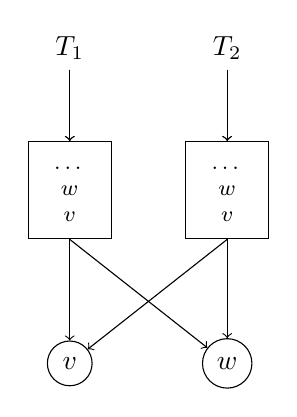
\begin{tikzpicture}
      \node (t1) at (-1,0) {$T_1$};
      \node (t2) at (1,0)  {$T_2$};
      \node (v) [draw,shape=circle] at (-1,-4) {$v$};
      \node (w) [draw,shape=circle] at (1,-4)  {$w$};

      \node (bt1) [draw] at (-1,-1.8) {\footnotesize\begin{tabular}{c} \ldots \\\midrule $w$ \\\midrule $v$ \end{tabular}};
      \node (bt2) [draw] at (1,-1.8) {\footnotesize\begin{tabular}{c} \ldots \\\midrule $w$ \\\midrule $v$ \end{tabular}};

      \draw [->] (t1) -- (bt1);
      \draw [->] (t1) -- (bt1);
      \draw [->] (t2) -- (bt2);
      \draw [->] (t2) -- (bt2);

      \draw [->] (bt1.south) -- (v);
      \draw [->] (bt1.south) -- (w);
      \draw [->] (bt2.south) -- (v);
      \draw [->] (bt2.south) -- (w);
    \end{tikzpicture}
    \caption{Total Store Order}
  \end{subfigure}
  \begin{subfigure}{0.3\textwidth}
    \centering
    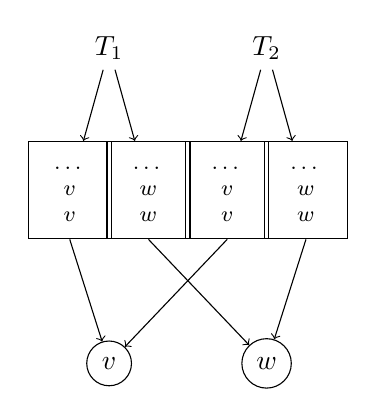
\begin{tikzpicture}
      \node (t1) at (-1,0) {$T_1$};
      \node (t2) at (1,0)  {$T_2$};
      \node (v) [draw,shape=circle] at (-1,-4) {$v$};
      \node (w) [draw,shape=circle] at (1,-4)  {$w$};

      \node (bt1v) [draw] at (-1.5,-1.8) {\footnotesize\begin{tabular}{c} \ldots \\\midrule $v$ \\\midrule $v$ \end{tabular}};
      \node (bt1w) [draw] at (-0.5,-1.8) {\footnotesize\begin{tabular}{c} \ldots \\\midrule $w$ \\\midrule $w$ \end{tabular}};
      \node (bt2v) [draw] at (0.5,-1.8) {\footnotesize\begin{tabular}{c} \ldots \\\midrule $v$ \\\midrule $v$ \end{tabular}};
      \node (bt2w) [draw] at (1.5,-1.8) {\footnotesize\begin{tabular}{c} \ldots \\\midrule $w$ \\\midrule $w$ \end{tabular}};

      \draw [->] (t1) -- (bt1v);
      \draw [->] (t1) -- (bt1w);
      \draw [->] (t2) -- (bt2v);
      \draw [->] (t2) -- (bt2w);

      \draw [->] (bt1v.south) -- (v);
      \draw [->] (bt1w.south) -- (w);
      \draw [->] (bt2v.south) -- (v);
      \draw [->] (bt2w.south) -- (w);
    \end{tikzpicture}
    \caption{Partial Store Order}
  \end{subfigure}
  \caption{Example of write buffering for two threads and two \texttt{CRef}s.}
  \label{fig:wb}
\end{figure}

We divide concurrency operations into three categories: \emph{synchronised}
operations impose a \emph{memory barrier}, which commits all buffered writes;
\emph{partially synchronised} operations commit one or more buffered writes to
the same \verb|CRef|; and \emph{unsynchronised} operations never cause a commit.

\paragraph{Phantom Threads}
In a sequentially consistent memory model, the set of runnable threads is
exactly the set of threads created by forking which are not blocked.  Under
relaxed memory, however, this is not the case.  For each write buffer, we
introduce one \emph{phantom thread}.  When scheduled, a phantom thread will
commit the oldest write in its corresponding buffer.

This may seem like an odd approach: why create new threads to model relaxed
memory?  The advantage is that systematic concurrency testing techniques assume
there is only one source of nondeterminism: the scheduler.  If a second source
is added, such as when writes are committed, it is difficult to integrate this
with existing algorithms.  By using phantom threads, the two sources of
nondeterminism are unified, and existing algorithms just work.  We take this
approach from \cite{zhang2015}.

\section{Testing Concurrent Programs}
\label{sec:dejafu-testing}

\dejafu{} uses a combination of dynamic partial-order reduction and
schedule bounding to test programs, by default.  Controlled random
scheduling using a fixed number of executions is also available.  To
make the tool easier to use, we provide a collection of different
testing functions, with varying levels of detail exposed, hoping that
the defaults will suffice for most users.  At one end of the scale we
have the \verb|autocheck| function, which looks for deadlocks,
uncaught exceptions in the main thread, and nondeterminism.  At the
other end of the scale is the \verb|dejafuDiscard| function which
exposes all the controls.

A \dejafu{} test has the following components:

\begin{itemize}
\item The testing algorithm to use plus any configuration it needs.
  The default is DPOR with schedule bounding.
\item A function to optionally discard results or traces as they are
  produced, and so not considering them when determining if the test
  passes.  This is a concession to performance: execution traces can
  take up a lot of memory, but typically we are only interested in a
  subset of them.
\item The memory model.  The default is total store order (TSO), as it
  is closest to the behaviour of an x86 processor\cite{owens2009},
  which is what the user probably has.
\item The \verb|MonadConc| action to test.
\item A named predicated, where a predicate is a function from the
  final list of results and traces to an indication of success or
  failure with an optional list of failing traces to display to the
  user.
\end{itemize}

\paragraph{Dependency Relation}
Correct DPOR relies on a dependency relation between pairs of actions
in a schedule trace.  This relation may be pessimistic, but cannot be
optimistic.  A pessimistic relation could claim that two actions are
related when they do not affect each other; an optimistic relation
could claim that two actions are unrelated when they do affect each
other.  A pessmistic relation may lead to exploring redundant
schedules, an optimistic relation may lead to missing distinct ones.

For ease of explanation, DPOR algorithms in the literature are
presented for small languages.  A paper will typically start with a
sentence like ``we assume a core concurrent language of reads and
writes to shared variables, and locks.''  The Haskell concurrency API
is richer than this, and the implicit dependencies between actions
(such as which actions impose a memory barrier) are not documented.
The dependency relation we now use in \dejafu{} was derived by running
small test cases many thousands of times.

We express our dependency relation in three parts: a relation on
\emph{thread actions}, which are entries in the trace; a relation on
\emph{thread action} and \emph{lookahead values}, which are forecasts
of what a thread will do, available to the scheduler; and a relation
on \emph{action types}, a simplification of thread actions.  Thread
actions contain more information than lookahead values, which contain
more information than action types.  We use this layered approach to
make use of this extra information to improve dependency detection
where possible.  \Cref{lst:deprel-simp} shows a simplified view of our
relations.  \Cref{app:deprel} shows the full dependency relation.

\begin{listing}
  \begin{minted}{haskell}
dependent :: ThreadId -> ThreadAction -> ThreadId -> ThreadAction -> Bool
dependent tid1 ta1 tid2 ta2
  | ...       = True
  | ...       = False
  | otherwise = dependent' tid1 ta1 tid2 (rewind ta2) &&
                dependent' tid2 ta2 tid1 (rewind ta1)

dependent' :: ThreadId -> ThreadAction -> ThreadId -> Lookahead -> Bool
dependent' tid1 ta tid2 lh
  | ...       = True
  | ...       = False
  | otherwise = dependentActions (simplifyAction    ta)
                                 (simplifyLookahead lh)

dependentActions :: ActionType -> ActionType -> Bool
dependentActions = ...
  \end{minted}
  \caption{A simplified view of the \dejafu{} dependency relations.}\label{lst:deprel-simp}
\end{listing}

For our dependency relation to be correct, we require some consistency
rules:

\begin{description}
\item[Commutativity (1)]
  $\mathrm{dependent}~x~y = \mathrm{dependent}~y~x$
\item[Commutativity (2)]
  $\mathrm{dependentActions}~x~y = \mathrm{dependentActions}~y~x$
\item[Consistency (1)]
  $\mathrm{dependent}~x~(t,y) \Rightarrow \mathrm{dependent'}~x~(t, \mathrm{rewind}~y)$
\item[Consistency (2)]
  $\mathrm{simplifyLookahead} = \mathrm{simplifyAction} \circ \mathrm{rewind}$
\end{description}

We establish these conditions through the syntactic structure of the
implementation.  Each function is a straightforward enumeration of
cases with attached side-conditions, which makes commutativity
apparent.  The more pessimistic \verb|dependent'| function is similar
to the more accurate \verb|dependent| function, but with less
information available, which makes consistency apparent.  We also
include these properties in the \dejafu{} testsuite to ensure they are
not inadvertently broken.

Through the lens of \verb|dependentActions|, Haskell is a small
concurrent language with synchronised and unsynchronised shared
variables and memory barriers.  The other cases which are handled by
\verb|dependent| and \verb|dependent'| are: lifted \verb|IO| actions,
exceptions, STM transactions, and getting and setting the number of
capabilities.

\paragraph{Sleep Sets}
The sleep set optimisation is a complementary approach to
DPOR\cite{flanagan2005,godefroid1996} which we use to further reduce
schedules explored.  The intuition is as follows: if we have a choice
of two scheduling decisions, $t_{1}$ and $t_{2}$, after trying out
$t_{1}$ there is no point in making the sequence of decisions
$t_{2}t_{1}$ unless $t_{1} \dependent t_{2}$.  This is because all
states reachable from $t_{1}$ have already been explored, so the only
way a new state could arise is if $t_{1}$ had a different effect, and
that is what it means for two transitions to be dependent.

Formally, we augment each state $s$ with a \emph{sleep set}, these are
the transitions enabled in $s$ but which we will not make.  The
initial state has an empty sleep set.  Let $T$ be the transitions that
have been selected to be explored from $s$.  We proceed as follows:
take a transition $t_{1}$ out of $T$.  The sleep set associated with
the state reached after executing $t_{1}$ from $s$ is the sleep set
associated with $s$ with all transitions that are dependent with
$t_{1}$ removed.  Let $t_{2}$ be a second transition taken out of $T$.
The sleep set associated with the state reached after executing
$t_{2}$ from $s$ is the sleep set associated with $s$ augmented with
$t_{1}$, minus all transitions that are dependent with $t_{2}$.  We
continue until all transitions in $T$ have been explored, at each step
adding the previously taken transitions to the sleep set of the new
state, and removing the dependent transitions.

\paragraph{Schedule Bounding}
\dejafu{} supports pre-emption bounding\cite{musuvathi2007}, fair
bounding\cite{musuvathi2008}, and length bounding.  Fair and length
bounding allow the testing of cyclic or potentially infinite
state-spaces, at the cost of potentially confusing the user by
aborting the execution of their program when it is still runnable.
All three bounds are enabled by default, but can be selectively
disabled or customised.

\paragraph{Daemon Threads}
A daemon thread is a thread which is automatically killed after the
last non-daemon thread terminates.  They do not prevent termination of
the program.  In Haskell, every thread other than the main thread is a
daemon thread, so as soon as it terminates the whole program
terminates.  This is a problem for DPOR, as it makes the last action
of the execution dependent with everything else in the program!

Consider this small example program:

\begin{minted}{haskell}
main = do
  v <- newEmptyMVar
  fork (myThreadId >> putMVar v "hello world")
  tryReadMVar v
\end{minted}

There are two possible results: \verb|Nothing|, and
\verb|Just "hello world"|, we would like to see both of these.
However, there is no dependency between \verb|myThreadId| and
\verb|tryReadMVar|, so if the deterministic scheduler used favours the
main thread, we may not see the second execution.  Introducing a
dependency between the last action of the execution and everything
else solves this.  Now consider this example:

\begin{minted}{haskell}
main = do
  v <- newEmptyMVar
  fork (myThreadId >> myThreadId >> putMVar v "hello world")
  tryReadMVar v
\end{minted}

The forked thread now performs two calls to \verb|myThreadId|.  If the
\verb|tryReadMVar| happens after the second, we get the same result as
if it happened after the first.  Normally, DPOR would prevent this
redundancy, but by introducing a dependency between the final action
and everything else, we have told the algorithm that it is \emph{not}
redundant!  In general, introducing a dependency like this will lead
to many redundant executions which we would otherwise avoid.

The solution we adopt is to change the deterministic scheduler.  If
the scheduler has a choice of actions, where one or more will cause
the main thread to terminate, it makes its choice as usual, and then
records every other decision as a backtracking point.  By ensuring
that every other decision is tried at least once, we do not need to
introduce an additional dependency between the final action of the
main thread and everything else, and can just let DPOR do its job as
usual.

\section{Soundness and Completeness}
\label{sec:dejafu-correctness}

Correctness for \dejafu{} breaks down along a natural separation in
the theory: correctness of a single execution of a concurrent program,
and correctness of the testing framework around this which discovers
new executions.  We can state correctness as ``nothing is missed and
nothing is made up,'' or:

\begin{description}
\item[Soundness] \dejafu{} only reports results of the program which
  could arise under normal execution.
\item[Compleness] \dejafu{} reports all results of the program which
  could arise under normal execution, taking any schedule bounds into
  account.
\end{description}

There is also the concern of correctness of the implementation with
respect to the theory.  We do not concern ourselves with that issue in
this thesis, only noting that humans are fallible and that there have
been bugs in \dejafu{} before now.  There are almost certainly still
bugs.  Whenever a bug is discovered, a test reproducing it is added to
the testsuite and the underlying issue is fixed.

\subsection{Correct Execution}

Correctness of execution asks whether the result of an arbitrary
execution of \dejafu{}'s testing implementation can be obtained in
reality; and, furthermore, do all real-world executions correspond to
a possible execution under \dejafu{}?  Both of these come with the
caveat that the behaviour can be different, as long as this difference
can't be observed.

\paragraph{Program Behaviour}
There is no standard for concurrent Haskell, there is only what GHC
provides.  The behaviour of many operations is clear, but not so for
others.  \verb|CRef| operations are particularly complicated, as their
behaviour depends on the underlying memory model, which is
unspecified.  We chose TSO, but ignore the possibility that the GHC
optimiser or code generator could affect the memory model.

We justify the correctness of our implementation with comprehensive
testing: there are many test cases, checking that \dejafu{} exhibits
behaviours which we consider realistic.  The relaxed memory
implementation is particularly difficult to test, for that we have a
collection of \emph{litmus tests} which we can evaluate many thousands
of times using \verb|IO| and compare to the results \dejafu{}
produces.

Furthermore, there are some intentional semantic differences for
practical concerns.  For example, GHC can sometimes detect deadlocks
involving only a subset of the threads, and throw an exception to the
threads signalling this.  We cannot do this.

So the behaviour of \dejafu{} is not correct, but we hope it is as
close as can reasonably be achieved.

\paragraph{Possible Executions}
Our stepwise execution of concurrent programs allows a scheduling
decision to be made between each primitive action, which doesn't
correspond to how GHC handles scheduling:

\begin{bquote}{Control.Concurrent module documentation\footnote{\url{https://hackage.haskell.org/package/base-4.10.0.0/docs/Control-Concurrent.html\#g:13}}}
  GHC implements pre-emptive multitasking: the execution of threads
  are interleaved in a random fashion.  More specifically, a thread may
  be pre-empted whenever it allocates some memory, which unfortunately
  means that tight loops which do no allocation tend to lock out other
  threads (this only seems to happen with pathological benchmark-style
  code, however).
\end{bquote}

So there are executions involving the pre-emption of the evaluation of
non-terminating expressions which are possible under GHC but not under
\dejafu{}.  Whether this can be used to produce different outputs is
unclear.

\subsection{Correct Testing}

Correctness of testing asks whether the schedule prefixes generated by
the DPOR machinery are valid; and, furthermore, are there any possible
results for which no schedule will be generated?  This is different to
the testing framework generating every schedule, as that is precisely
what DPOR tries to avoid.

\paragraph{Prefix Validity}
Executions are stored internally as a stack, shown in \cref{lst:dpor}.
The sequence of thread IDs corresponding to this stack represents a
complete execution of the program.  There is a unique initial state,
where only the initial thread is runnable and nothing has been done.

\begin{listing}
  \begin{minted}{haskell}
data DPOR = DPOR
  { dporRunnable :: Set ThreadId
  -- ^ What threads are runnable at this step.
  , dporTodo     :: Map ThreadId Bool
  -- ^ Follow-on decisions still to make, and whether that decision
  -- was added conservatively due to the bound.
  , dporNext     :: Maybe (ThreadId, DPOR)
  -- ^ The next decision made. Executions are explored in a
  -- depth-first fashion, so this changes as old subtrees are
  -- exhausted and new ones explored.
  , dporDone     :: Set ThreadId
  -- ^ All transitions which have been taken from this point,
  -- including conservatively-added ones.
  , dporSleep    :: Map ThreadId ThreadAction
  -- ^ Transitions to ignore (in this node and children) until a
  -- dependent transition happens.
  , dporTaken    :: Map ThreadId ThreadAction
  -- ^ Transitions which have been taken, excluding
  -- conservatively-added ones. This is used in implementing sleep
  -- sets.
  } deriving (Eq, Show)
  \end{minted}
  \caption[The \dejafu{} DPOR state.]{The DPOR state is a stack of scheduling decisions.}\label{lst:dpor}
\end{listing}

There are some basic well-formedness properties associated with a
\verb|DPOR| value: every thread in the to-do set is runnable; every
thread in the done set is runnable; the done and to-do sets are
disjoint; no thread in the sleep set is also in the done set; the
taken set is the done set excluding the sleep set; the next-taken
decision (if there is one) is in the runnable set and not in the to-do
or sleep sets; and these properties hold recursively.

A generated schedule prefix is one of the longest sequence of taken
decisions followed by a single to-do decision possible.  This
corresponds to a depth-first search of the space of schedules.  As
long as the well-formedness properties hold, and the runnable sets are
correctly recorded during execution, then a generated schedule prefix
will be valid.

\paragraph{Schedule Completeness}
The simplest notion of completeness of interest here is that for all
results possible by executing a given program, the DPOR machinery can
give that result.  However, as schedule bounding is involved, this is
not the case.  So we have two slightly different notions of
completeness:

\begin{enumerate}
\item When all schedule bounds are disabled, all possible results show
  up under testing.
\item For all sets of bounds, all results possible subject to those
  bounds show up under testing with the same bounds.
\end{enumerate}

Property (2) implies property (1).  We use \cite{coons2013} as our
core DPOR algorithm, which establishes property (2).

\section{Case Studies}
\label{sec:dejafu-casestudies}

Three case studies are discussed, two of which are from pre-existing
libraries which have been modified to use the \verb|MonadConc|
abstraction.  A known bug is reproduced in the \package{auto-update}
library.  Then, there is a bug which arose unintentionally in the
implementation of a library for expressing parallel search problems.
Finally, one of the schedulers in the \package{monad-par} package is
tested.

\subsection{The auto-update Package}

\begin{listing}
  \begin{minted}{haskell}
data UpdateSettings a = UpdateSettings
    { updateFreq           :: Int
    , updateSpawnThreshold :: Int
    , updateAction         :: IO a
    }

defaultUpdateSettings :: UpdateSettings ()
defaultUpdateSettings = UpdateSettings
    { updateFreq           = 1000000
    , updateSpawnThreshold = 3
    , updateAction         = return ()
    }

mkAutoUpdate :: UpdateSettings a -> IO (IO a)
mkAutoUpdate us = do
    currRef      <- newIORef Nothing
    needsRunning <- newEmptyMVar
    lastValue    <- newEmptyMVar

    void $ forkIO $ forever $ do
        takeMVar needsRunning

        a <- catchSome $ updateAction us

        writeIORef currRef $ Just a
        void $ tryTakeMVar lastValue
        putMVar lastValue a

        threadDelay $ updateFreq us

        writeIORef currRef Nothing
        void $ takeMVar lastValue

    return $ do
        mval <- readIORef currRef
        case mval of
            Just val -> return val
            Nothing -> do
                void $ tryPutMVar needsRunning ()
                readMVar lastValue

catchSome :: IO a -> IO a
catchSome act = catch act $
  \e -> return $ throw (e :: SomeException)
  \end{minted}
  \caption{The implementation of the auto-update package.}\label{lst:example-autoupdate}
\end{listing}

The \textbf{auto-update} library runs tasks periodically, but only if
needed.  For example, a single worker thread may get the time every
second and store it to a shared \verb|CRef|, rather than have many
threads starting within a second of each other all get the time
independently.  Despite the core functionality being simple, a race
condition was noticed by users inspecting the code in October 2014.

The entire implementation, excluding comments and imports, is
reproduced in \cref{lst:example-autoupdate}.  The \verb|mkAutoUpdate|
function spawns a worker thread, which performs the update action at
the given frequency, only if the \verb|needsRunning| flag has been
set.  It returns an action to attempt to read the current result, if
necessary blocking until there is one.  The transformation to the
\verb|MonadConc| typeclass is straightforward.

The race condition occurs if the reading thread is pre-empted by the
worker thread after putting into \verb|needsRunning|, and does not run
again until after the delay has passed.  In this case the worker
thread can become blocked on taking for a second time from
\verb|needsRunning|.  The reader thread will be unable to read from
\verb|lastValue| as the worker thread emptied it as the last action it
performed.  The race condition can be exhibited with the following
test:

\begin{minted}{haskell}
test :: MonadConc m => m ()
test = join (mkAutoUpdate defaultUpdateSettings)
\end{minted}

This test was chosen as it is one of the simplest things a user may
wish to do with the library: to create the worker, and to then read
the computed value.  The output of testing shows the different results
that were found, with a sample trace leading to each one:

\begin{minted}{text}
> autocheck test
[fail] Never Deadlocks (checked: 5)
        [deadlock] S0--------S1---------S0-
[pass] No Exceptions (checked: 55)
[fail] Consistent Result (checked: 54)
        () S0--------S1------P0--

        [deadlock] S0--------S1---------S0-
\end{minted}

The \verb|autocheck| function is used to search for deadlocks,
uncaught exceptions in the main thread, and nondeterminism in
results. In this display, ``S$n$'' indicates that thread $n$ began
executing after the prior one terminated, blocked, or yielded; and
``P$n$'' indicates that thread $n$ pre-empted the prior one.

To read this trace, it is helpful to look at the ``S'' points, rather
than to count the steps.  Using this tactic, we see that a deadlock
occurs if thread 0 (the initial thread) runs until it blocks (which is
the \verb|readMVar lastValue| call), then thread 1 (the worker thread)
runs until it blocks (the second time \verb|takeMVar needsRunning| is
reached).  At this point the initial thread is runnable, as it was
unblocked by the write to \verb|lastValue|.  The initial thread is
scheduled, and immediately blocks because the worker thread took the
value.  Both threads are now blocked, and so the computation is
deadlocked.

This deadlock may arise in any use of the library, as it depends only
on the timing of the delay, and not on the computation performed.  If
the call to \verb|threadDelay| completes before the reading thread has
resumed execution, this situation will arise.  Despite this bug being
rather simple, not requiring any pre-emptions at all to trigger, it
arose in practice.  How easy it is to make mistakes when implementing
concurrent programs!

\subsection{Search Party}

The \textbf{Search Party}\footnote{\url{https://github.com/barrucadu/search-party}}
library supports speculative parallelism in generate-and-test search
problems.  It is motivated by the consideration that if multiple
acceptable solutions exist, it may not matter which one is returned.
In early versions of the library, only single results could be
returned, but support for returning all results was later added,
incorrectly, introducing a bug.

The library provides a collection of combinators used to express a
generate-and-test problem, which are executed in using a concurrent
producer/consumer pattern.  One worker thread is created for each
capability, which share a list of work items and communicate results
back to the main thread.

A key piece of worker loop is as follows:

\begin{minted}{haskell}
case maybea of
  Just a -> do
    atomically $ do
      val <- tryTakeTMVar res
      case val of
        Just (Just as) -> putTMVar res $ Just (a:as)
        _ -> putTMVar res $ Just [a]
    unless shortcircuit $
      process remaining res
  Nothing -> process remaining res
\end{minted}

Here \verb|maybea| is a value indicating whether the computation just
evaluated was successful.  A \verb|TMVar| (used by the
\verb|tryTakeTMVar| and \verb|putTMVar| functions) is a \verb|TVar|
containing a \verb|Maybe| value, which aborts the transaction if it
fails.  The result is a similar type to the \verb|MVar|, but
composable.  The intended behaviour of this code that, if a
computation is successful, its result is added to the list in the
\verb|res| \verb|TMVar|.  This \verb|TMVar| is exposed indirectly to
the user of the library, as it is blocked upon when the result of the
search is requested.

Upon introducing this new functionality, tests for it were added to
the testsuite:\footnote{The \texttt{representative} function picks
  only one trace for each unique result.}

\begin{minted}{haskell}
checkResultLists :: Eq a => Predicate [a]
checkResultLists = representative (alwaysTrue2 check) where
  check (Right as) (Right bs) = as `elem` permutations bs
  check a b = a == b
\end{minted}

This \dejafu{} predicate checks that all result lists are equal, up to
ordering.  Given this predicate, we can see the problem:

\begin{minted}{text}
> let test xs = takeStream (length xs) =<< xs @! const True
> dejafu (test [0..2]) ("Result Lists", checkResultLists)
[fail] Result Lists (checked: 38)
        [] S0------S1-----S0-------

        [0] S0------S1-----S0---P3------------S0-------

        [0,1] S0------S1-----S0---P3------------S0--P3------S0--------

        [1] S0------S1-----S0---P2-P3------------S0-------
\end{minted}
%>> - emacs does some silly highlighting after the << above

The \verb|@!| operator is a concurrent filter, with the order of
results nondeterministic.  The problem was a lack of any indication
that a list-producing computation had finished.  As results were
written directly to the \verb|TMVar|, partial result lists could be
read depending on how the worker threads and the main thread were
interleaved.

In this case, fixing the failure did not require any interactive
debugging.  Only one place had been modified in introducing the new
functionality, and the bug was found by re-reading the code with the
possibility of error in mind.  However, the ability to produce a test
case which reliably reproduces the problem gives confidence that it
will not be accidentally reintroduced.

\FloatBarrier
\subsection{The Par Monad}

\begin{listing}
  \begin{sublisting}{\textwidth}
    \begin{minted}{haskell}
makeScheds :: Int -> IO [Sched]
makeScheds main = do
   workpools <- replicateM numCapabilities $ R.newQ
   rngs <- replicateM numCapabilities $ Random.create >>= newHotVar
   idle <- newHotVar []
   sessionFinished <- newHotVar False
   sessionStacks   <- mapM newHotVar
     (replicate numCapabilities [Session baseSessionID sessionFinished])
   activeSessions  <- newHotVar S.empty
   sessionCounter  <- newHotVar (baseSessionID + 1)
   let allscheds = [ Sched { no=x, idle, isMain=(x==main), workpool=wp,
                             scheds=allscheds, rng=rng, sessions=stck
                             sessionCounter, activeSessions
                           }
                   | x   <- [0 .. numCapabilities-1]
                   | wp  <- workpools
                   | rng <- rngs
                   | stck <- sessionStacks
                   ]
   return allscheds
    \end{minted}
    \caption{Original}\label{lst:example-parmonad-sched-orig}
  \end{sublisting}

  % [layout hack]: no gap between the listings otherwise
  \vspace{2.5em}

  \begin{sublisting}{\textwidth}
    \begin{minted}{haskell}
makeScheds :: (MonadConc m, MonadIO m) => Int -> m [Sched m]
makeScheds main = do
   numCapabilities <- getNumCapabilities
   workpools <- replicateM numCapabilities $ liftIO R.newQ
   let rng i = liftIO (Random.initialize (V.singleton $ fromIntegral i))
   rngs <- mapM (\i -> rng i >>= newHotVar) [0..numCapabilities]
   idle <- newHotVar []
   sessionFinished <- newHotVar False
   sessionStacks   <- mapM newHotVar
     (replicate numCapabilities [Session baseSessionID sessionFinished])
   activeSessions  <- newHotVar S.empty
   sessionCounter  <- newHotVar (baseSessionID + 1)
   let allscheds = [ Sched { no=x, idle, isMain=(x==main), workpool=wp,
                             scheds=allscheds, rng=rng, sessions=stck
                             sessionCounter, activeSessions
                           }
                   | x   <- [0 .. numCapabilities-1]
                   | wp  <- workpools
                   | rng <- rngs
                   | stck <- sessionStacks
                   ]
   return allscheds
    \end{minted}
    \caption{\dejafu{}}\label{lst:example-parmonad-sched-dejafu}
  \end{sublisting}
  \caption{The monad-par ``direct'' scheduler initialisation.}\label{lst:example-parmonad-sched}
\end{listing}

The \package{monad-par} library\cite{marlow2011} provides a
traditional-looking concurrency abstraction, giving the programmer
threads and mutable state, however it maintains determinism by
restricting its shared variables to one write, and read operations
block until a value has been written.  These shared \verb|IVar|
variables are used to implement futures, rather than general mutable
state.  The package uses a work-stealing scheduler running on multiple
operating system threads, fully evaluating values on their own threads
before inserting them into an \verb|IVar|.  Despite its limitations,
the library can be effective in speeding up pure code.

The library provides several different schedulers.  We ported the
``direct'' scheduler to the \verb|MonadConc| typeclass so it could be
tested.  This resulted in two files needing change.  This was a
straightforward and compiler-driven refactoring.  Changing function
types to reference \verb|MonadConc| rather than \verb|IO| led to
compiler errors showing where the next changes needed to be made.  We
iterated this process of fixing errors and recompiling until the
library compiled once more.

Some simplifications were made in the conversion process:

\begin{itemize}
\item The scheduler uses the \package{mwc-random} library to fairly
  distribute work to the worker threads.  By default, the initial seed
  is an effectively random value.  As systematic testing requires that
  the scheduler be the only source of nondeterminism, we fixed the
  random seed.
\item Behaviour of the scheduler can be configured using cpp, but we
  only ported the default configuration.
\end{itemize}

\Cref{lst:example-parmonad-sched} shows the original and converted
scheduler initialisation code.  As can be seen, they are similar, even
though this is a core component of a rather sophisticated library,
where the types have been changed.  \Cref{tbl:example-parmonad-diff}
breaks down the changes across both files.  Code changes are broken
down into ``renames,'' where the \textbf{concurrency} library simply
provides a different name for a function, and ``logic,'' where that
was not the case.  The logic changes were all places where a call to
\verb|liftIO| or \verb|lift| was now necessary, and inserting uses of
\verb|getNumCapabilities|.

\begin{table}
  \centering
  \begin{tabular}{l|rr} \toprule
    & Direct.hs & DirectInternal.hs \\ \midrule
    Language extensions & 1 & 0 \\
    Module imports & 6 & 1 \\
    Type definitions & 7 & 13 \\
    Type signatures & 32 & 7 \\
    Function renames & 13 & 5 \\
    Logic changes & 16 & 0 \\ \midrule
    \emph{Total} & 75 & 26 \\ \bottomrule
  \end{tabular}
  \caption{Breakdown of changes to port the monad-par ``direct'' scheduler.}\label{tbl:example-parmonad-diff}
\end{table}

No deadlock or nondeterminism was discovered, with a variety of
initial random seeds tried.

\section{Evaluation}
\label{sec:dejafu-evaluation}

A tool is effectively useless if it is too difficult to use.  The main
obstacle to the use of \dejafu{} is existing libraries which use
\verb|IO|; a programmer cannot simply use \verb|liftIO| everywhere,
without sacrificing completeness in all but trivial examples.
Ideally, existing libraries would be modified to support the
\verb|MonadConc| abstraction.  However, this does not seem a likely
short-term goal, and so a more promising way to approach the problem
is to provide feature complete alternatives to existing libraries.  As
adapting code to \verb|MonadConc| is often straightforward, as seen in
the Par monad case study, this is a viable short-term solution.

A second, more tractable, problem is integration with existing testing
frameworks; using \dejafu{} for little stand-alone programs is all
well and good, but to take off, it must be easy to use in the testing
context people are already familiar with.

\paragraph{Users}
Although \dejafu{} is a small one-man project, it does have some users
and contributors.  Seven users have opened issues on the GitHub issue
tracker\footnote{\url{https://github.com/barrucadu/dejafu/issues}}; a
further three have asked me for help over IRC and email; and five have
made small
contributions\footnote{\url{https://github.com/barrucadu/dejafu/graphs/contributors}}.
Two features came directly from user requests, motivated by
performance concerns in large test cases: random scheduling; and the
ability to discard uninteresting results as they are discovered,
before evaluating the predicate at the end.

Tweag I/O\footnote{\url{http://www.tweag.io/}}, a research and
development company based in Paris, are using \dejafu{} as part of
their work on the SAGE
project\footnote{\url{http://www.sagestorage.eu/}} on developing
storage systems for future supercomputers.  They cannot share specific
details of their work for commercial reasons, but one developer had
this to say:

\begin{bquote}{Email correspondence about a slow test}
  Regarding the test case: we have an implementation of a distributed
  storage cluster, with possibly many nodes and parallel requests.
  The storage system itself is composed of several layers, which can
  be stacked on top of one another.  There is a lot of asynchronicity
  involved.  As per the tests themselves, I am testing parallel
  requests over different objects, etc.

  I'd like to add that dejafu tests are by far the most reliable tests
  in our suite, in my experience - I am yet to see a concurrency bug
  that they didn't spot, while some other tests missed them!
\end{bquote}

\subsection{Richness of the Abstraction}

As we noted earlier, there are three main areas which we do not
currently aim to support with \dejafu{}:

\begin{itemize}
\item Blocking a thread until a file descriptor becomes available, as
  this introduces an additional source of nondeterminism.
\item Throwing an exception to a thread if it becomes deadlocked, as
  we cannot reliably detect deadlock involving only a subset of
  threads without support from the garbage collector.
\item Querying which capability (OS thread) a Haskell thread is
  running on, as this introduces an additional source of
  nondeterminism.
\end{itemize}

Introducing additional sources of nondeterminism into an SCT model is
difficult.  Simply introducing additional threads to model the
nondeterminism can cause an explosion of schedules tested, which is
unsatisfactory.  In this way, \verb|MonadConc| will always be limited
to what \dejafu{} can reasonably support.

However we also push back the barrier of what \dejafu{} supports.
Bound threads, Haskell threads which always run on the same unique OS
thread, were once out of scope as well.  This made it impossible to
use some C libraries with \verb|MonadConc|.  Now we have a prototype
implementation\footnote{\url{https://github.com/barrucadu/dejafu/issues/126}}
which shows promise, and which we intend to release.

\dejafu{} does not aim to support the above three areas because we
believe that the desire for this functionality does not outweigh the
implementation cost.  If that belief changes, we will look for a way.

\subsection{Porting and Writing Code}

We saw in the \textbf{monad-par} example that porting complex code to
the \verb|MonadConc| abstraction is not necessarily a difficult
process.  However, this is not always the case.  Recently a user tried
to port a logging abstraction they made to \verb|MonadConc|.  The
original code looked like this:

\begin{minted}{haskell}
instance MonadLogger (LoggerT STM) where -- ...
instance MonadLogger (LoggerT IO) where -- ...
\end{minted}

Expressing this with \verb|MonadConc| and \verb|MonadSTM| is less
straightforward, as constraints do not factor into instance selection.
So these two instances overlap:

\begin{minted}{haskell}
instance MonadSTM  m => MonadLogger (LoggerT m) where -- ...
instance MonadConc m => MonadLogger (LoggerT m) where -- ...
\end{minted}

After some work, we introduced new types to disambiguate between the
two cases, and ended up with something like this:

\begin{minted}{haskell}
instance MonadSTM  m => MonadLogger (LoggerT (IsSTM  m)) where -- ...
instance MonadConc m => MonadLogger (LoggerT (IsConc m)) where -- ...
\end{minted}

Where \verb|IsSTM| and \verb|IsConc| are new types we introduced, with
their own \verb|MonadSTM| and \verb|MonadConc| instances.  The amount
of effort required to arrive at this solution led to the user
questioning whether classes like their \verb|MonadLogger| were even a
useful abstraction at all\footnote{\url{https://www.reddit.com/r/haskell/comments/7b1fbk/do_mtlstyle_effect_classes_really_pull_their/}}!
This is a good topic to think about, but it should not be prompted by
the effort of trying to use \dejafu{}.

So while porting code to the \verb|MonadConc| typeclass is often
simple when dealing with datatype and function definitions, it can be
more complicated when dealing with typeclasses.  It is not clear what
can be done to improve this matter.

\subsection{Library Alternatives}

There are popular Haskell libraries specifically for concurrency.  One
of these is the \package{async} library, for expressing asynchronous
computations.  This library is intended to be a higher-level and safer
way of expressing asynchronous computations than using threading and
mutable state directly.  It provides two main functions to execute an
action asynchronously:

\begin{minted}{haskell}
async     :: IO a -> IO (Async a)
withAsync :: IO a -> (Async a -> IO b) -> IO b
\end{minted}

Both of these fork the computation into a separate thread, returning
an \verb|Async| value, which can be blocked on to retrieve the result,
or used to kill the thread.  In addition, \verb|withAsync| kills the
thread if the inner action (which is run in the original thread)
completes first, to help prevent resource leaks.

There is a further abstraction atop \verb|Async|, called
\verb|Concurrently|, which has Functor, Applicative, and Alternative
instances, and represents an action which can be concurrently composed
with other actions.  The concurrency is achieved by having the
Applicative \verb|(<*>)| operator execute each action asynchronously.
There was once a Monad instance for \verb|Concurrently|, but it was
inconsistent with the Applicative
instance\footnote{\url{https://github.com/simonmar/async/pull/26}}.

This law-breaking could have been discovered through testing, but only
probabilistically.  If \textbf{async} were written using
\verb|MonadConc|, the relevant laws could have been specified as unit
tests and checked.  The bug might then have been caught before it
showed up in user code.  Indeed, the \dejafu{} testsuite contains this
invalid Monad instance and checks that the failure is caught.

The \textbf{concurrency} package, which provides \verb|MonadConc|,
includes an alternative to \textbf{async} using \verb|MonadConc|.
There is a test suite using \dejafu{}.  The test suite for
\textbf{async} itself just runs most tests a single time, although one
of them is run 1000 times.  Using \dejafu{} here to automatically seek
out interesting schedules is a much more principled approach then
repetition and hope.  Not all features of \textbf{async} are
supported, however.  As we do not currently support bound threads,
those functions that use them have been omitted.

This is just one library, and providing an alternative library people
will have to switch to is far from optimal.  However, until library
authors start to use \dejafu{} and \verb|MonadConc| directly, such
alternatives will be needed to answer the question ``Why should I use
this if I can't use it with anything I use already?''

\subsection{Tool Integration}

There are two popular libraries for unit testing in Haskell,
\package{HUnit} and \package{tasty}.  From the perspective of the
user, the libraries are similar, but from the perspective of the
implementer, they have different approaches to integration.  The
\package{hunit-dejafu} and \package{tasty-dejafu} packages provide
integration with both.

These packages provide a common set of testing functions, an analogue
of Test.DejaFu but constructing values representing individual tests
which the frameworks can run, rather than executing and printing
results directly.  The \package{test-framework} library is also in
common use, however it supports integration with \textbf{HUnit}, and
so needs no special support. of its own.

The \textbf{tasty} library is more featureful than \textbf{HUnit},
supporting progress reporting, giving a message on success as well as
failure, and command-line arguments.  The \textbf{tasty-dejafu}
package is similar to the \textbf{hunit-dejafu} package and does not
make use of these additional features.

\section{Conclusions}
\label{sec:dejafu-conclusions}

Although a commonly reported experience amongst Haskell programmers is
that ``if it compiles, it works'', there are times where it does
\emph{not} work.  A number of profiling and debugging tools exist,
typically requiring special runtime support.  Concurrency is a
particularly difficult area to get right, as everyone who has had to
move outside the realm of guaranteed determinism will know.  Yet there
are no debugging tools for concurrent Haskell programs.  We contribute
such a tool, at the cost of a programmer having to use a
generalisation of the familiar concurrency abstraction.

This work was inspired by attending a talk at INVEST
2014\footnote{\url{http://wp.doc.ic.ac.uk/verificationgroup/event/workshop-introduction-to-verification-and-testing-invest-2014/}}
by Paul Thompson, then a Ph.D student at Imperial College London, on
systematic concurrency testing, the talk mentioned tools for languages
like Java and C, but functional languages were not mentioned at all.
The questions to be answered, then, were:

\begin{itemize}
\item \textbf{Can concurrency testing techniques from the imperative
    and object-oriented worlds be applied in the functional world?}
  \hfill

  The answer to this would seem to be a resounding ``yes''.  There was
  some difficulty in implementing these techniques in a purely
  functional setting, as the algorithms are typically expressed in
  terms of mutable state, but this was overcome.

\item \textbf{Does the purely functional setting allow for new
    techniques to be developed?} \hfill

  At first we hoped that the lack of side-effects in evaluation,
  amongst other things, would allow for new techniques to be
  developed.  However, as concurrency testing explicitly cares about
  \emph{execution} rather than \emph{evaluation} (although these are
  one and the same in most languages), this does not seem to be the
  case.
\end{itemize}

In \cite{walker2015}, we asked if the cost of a programmer needing to
write their code in terms of \verb|MonadConc| rather than \verb|IO|
was too high, and would discourage people.  This is still a concern,
but with the development of libraries to integrate with or replace
others, we hope that the use of \dejafu{} will appear attractive
enough to overcome this.

The contributions of this work are:

\begin{itemize}
\item a generalisation of a large subset of the GHC concurrency
  abstraction;

\item a library called \dejafu{} for the systematic and random testing
  of concurrent Haskell programs, including those using relaxed-memory
  effects.
\end{itemize}
